\section{Ex.1 2 FLPs 12 EPNs}
\textbf{Ticktime influence on the Blacklist algorithm with one fail-over.}
\\~\\
The results of the experiment are shown in table ~\ref{table:Ex1MitchResults}. It shows that there is a linear line going up with the amount of TFs lost compared to ticktime. It also shows that the mean and standard deviation at ticktime 20 are round. This would be because of the ticktime being in sync with the heartbeat rate.

\begin{table}[h!]
\begin{tabular}{| l | l | l |}
\hline
Ticktime & Mean TF loss & Standard Deviation \\ \hline
5 & 2.16 & 0.49 \\ \hline
10 & 2.13 & 0.47 \\ \hline
15 & 3.08 & 0.2 \\ \hline
20 & 3.0 & 0 \\ \hline
25 & 3.52 & 0.51 \\ \hline
30 & 4.32 & 0.57 \\ \hline
35 & 4.13 & 0.79 \\ \hline
40 & 4.56 & 0.16 \\ \hline
\end{tabular}
\caption{Results of the TFs lost with 1 fail over using a cluster of Raspberry Pi's}
\label{table:Ex1MitchResults}
\end{table}

~\\ If we compare this to the previous experiment shown in table ~\ref{table:Ex1HeikoResults}, we can see that there is a small difference in the mean of the TFs lost, and some small variations in the standard deviation.

\begin{table}[h!]
\begin{tabular}{| l | l | l |}
\hline
Ticktime & Mean TF loss & Standard Deviation \\ \hline
5 & 1.24 & 0.4271 \\ \hline
10 & 1.84 & 0.731 \\ \hline
15 & 2.16 & 0.3666 \\ \hline
20 & 2.12 & 0.325 \\ \hline
25 & 2.708 & 0.4545 \\ \hline
30 & 3 & 0 \\ \hline
35 & 3.52 & 4.996 \\ \hline
40 & 3.76 & 0.4271 \\ \hline
\end{tabular}
\caption{Results of the TFs lost with 1 fail over using a cluster of Intel Xeons (van der Heijden, 2018, p. 36)}
\label{table:Ex1HeikoResults}
\end{table}

\section{Ex.2 2 FLPs 12 EPNs}
\textbf{Ticktime influence on the Blacklist algorithm with all but one fail-over.}
\\~\\
Table ~\ref{table:Ex2MitchResults} shows the lost TFs per ticktime/EPN ratio. For every extra EPN that is lost, the lost TFs increase in a linear motion. This is compliant with the previous experiment. These results are shown in table ~\ref{table:Ex2HeikoResults}. A histogram of ticktime 5 shown at ~\ref{Ex2Histogram} shows that the standard deviation is 0.9568.

\begin{table}[h!]
\resizebox{\textwidth}{!}{\begin{tabular}{| p{0.1\linewidth} | >{\centering}m{0.7cm} | >{\centering}m{0.7cm} | >{\centering}m{0.7cm} | >{\centering}m{0.7cm} | >{\centering}m{0.7cm} | >{\centering}m{0.7cm} | >{\centering}m{0.7cm} | >{\centering}m{0.7cm} | >{\centering}m{0.7cm} | >{\centering}m{0.7cm} | >{\centering}m{0.7cm} |}
\hline
Lost EPNs & 1 EPN & 2 EPNs & 3 EPNs & 4 EPNs & 5 EPNs & 6 EPNs & 7 EPNs & 8 EPNs & 9 EPNs & 10 EPNs & 11 EPNs \tabularnewline \hline
Ticktime &&&&&&&&&&& \tabularnewline \hline
5 & 2 & 2 & 2 & 2 & 2 & 3 & 3 & 3 & 4 & 4 & 5 \tabularnewline \hline
10 & 2 & 3 & 3 & 3 & 3 & 4 & 4 & 4 & 4 & 5 & 7 \tabularnewline \hline
15 & 3 & 3 & 3 & 3 & 4 & 4 & 4 & 5 & 6 & 7 & 9 \tabularnewline \hline
20 & 3 & 4 & 4 & 4 & 4 & 5 & 5 & 6 & 7 & 9 & 11 \tabularnewline \hline
25 & 4 & 4 & 4 & 4 & 5 & 5 & 6 & 7 & 9 & 10 & 13 \tabularnewline \hline
\end{tabular}}
\caption{Cumulative lost TFs by ticktime/EPN ratio with a flat sample size for the Blacklist algorithm}
\label{table:Ex2MitchResults}
\end{table}

\begin{table}[h!]
\resizebox{\textwidth}{!}{\begin{tabular}{| p{0.1\linewidth} | >{\centering}m{0.7cm} | >{\centering}m{0.7cm} | >{\centering}m{0.7cm} | >{\centering}m{0.7cm} | >{\centering}m{0.7cm} | >{\centering}m{0.7cm} | >{\centering}m{0.7cm} | >{\centering}m{0.7cm} | >{\centering}m{0.7cm} | >{\centering}m{0.7cm} | >{\centering}m{0.7cm} |}
\hline
Lost EPNs & 1 EPN & 2 EPNs & 3 EPNs & 4 EPNs & 5 EPNs & 6 EPNs & 7 EPNs & 8 EPNs & 9 EPNs & 10 EPNs & 11 EPNs \tabularnewline \hline
Ticktime &&&&&&&&&&& \tabularnewline \hline
5 & 1 & 2 & 2 & 2 & 2 & 2 & 2 & 3 & 3 & 3 & 4 \tabularnewline \hline
10 & 1 & 2 & 3 & 3 & 3 & 3 & 3 & 3 & 4 & 4 & 5 \tabularnewline \hline
15 & 1 & 3 & 3 & 3 & 3 & 3 & 4 & 4 & 4 & 5 & 7 \tabularnewline \hline
20 & 9 & 3 & 3 & 3 & 4 & 4 & 4 & 5 & 5 & 6 & 8 \tabularnewline \hline
25 & 11 & 3 & 4 & 4 & 4 & 4 & 5 & 5 & 6 & 7 & 9 \tabularnewline \hline
\end{tabular}}
\caption{Cumulative lost TFs by ticktime by lost EPNs (van der Heijden, 2018, p. 38)}
\label{table:Ex2HeikoResults}
\end{table}

\newpage

\begin{figure}[h!]
	\centering
	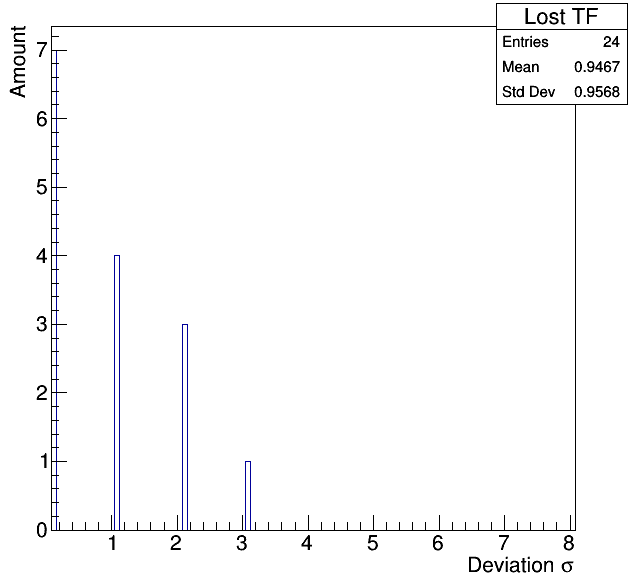
\includegraphics[scale=0.5]{./graphics/ex2_histogram.png}
	\caption{Histogram of the TF lost for ticktime 5}
	\label{Ex2Histogram}
\end{figure}

\newpage

\section{Ex.3 2 FLPs 12 EPNs}
\textbf{Ticktime influence on the Blacklist algorithm with all but one-fail over with random sample size.}
\\~\\
Compliant with the previous results, the TF loss to ticktime ratio rises in a linear line, with no absurdities along the way. The amounts are also negligibly different to the previous results. Results can be seen in table ~\ref{table:Ex3MitchResults} and table ~\ref{table:Ex3HeikoResults}. A histogram for ticktime 5 can be seen at ~\ref{fig:Ex3Histogram}. It shows a standard deviation of 1.569 for all the TFs lost in the entire run. 

\begin{table}[h!]
\resizebox{\textwidth}{!}{\begin{tabular}{| p{0.1\linewidth} | >{\centering}m{0.7cm} | >{\centering}m{0.7cm} | >{\centering}m{0.7cm} | >{\centering}m{0.7cm} | >{\centering}m{0.7cm} | >{\centering}m{0.7cm} | >{\centering}m{0.7cm} | >{\centering}m{0.7cm} | >{\centering}m{0.7cm} | >{\centering}m{0.7cm} | >{\centering}m{0.7cm} |}
\hline
Lost EPNs & 1 EPN & 2 EPNs & 3 EPNs & 4 EPNs & 5 EPNs & 6 EPNs & 7 EPNs & 8 EPNs & 9 EPNs & 10 EPNs & 11 EPNs \tabularnewline \hline
Ticktime &&&&&&&&&&& \tabularnewline \hline
5 & 1 & 2 & 2 & 2 & 3 & 3 & 3 & 3 & 4 & 4 & 5 \tabularnewline \hline
10 & 2 & 2 & 3 & 3 & 3 & 3 & 3 & 3 & 4 & 5 & 7 \tabularnewline \hline
15 & 3 & 3 & 3 & 3 & 4 & 4 & 4 & 5 & 6 & 7 & 9 \tabularnewline \hline
20 & 3 & 3 & 4 & 4 & 4 & 4 & 5 & 6 & 6 & 8 & 12 \tabularnewline \hline
25 & 4 & 4 & 4 & 4 & 4 & 5 & 6 & 7 & 8 & 10 & 13 \tabularnewline \hline
\end{tabular}}
\caption{Cumulative lost TFs by ticktime/EPN ratio with a random sample size for the Blacklist algorithm}
\label{table:Ex3MitchResults}
\end{table}

\begin{table}[htb]
\resizebox{\textwidth}{!}{\begin{tabular}{| p{0.1\linewidth} | >{\centering}m{0.7cm} | >{\centering}m{0.7cm} | >{\centering}m{0.7cm} | >{\centering}m{0.7cm} | >{\centering}m{0.7cm} | >{\centering}m{0.7cm} | >{\centering}m{0.7cm} | >{\centering}m{0.7cm} | >{\centering}m{0.7cm} | >{\centering}m{0.7cm} | >{\centering}m{0.7cm} |}
\hline
Lost EPNs & 1 EPN & 2 EPNs & 3 EPNs & 4 EPNs & 5 EPNs & 6 EPNs & 7 EPNs & 8 EPNs & 9 EPNs & 10 EPNs & 11 EPNs \tabularnewline \hline
Ticktime &&&&&&&&&&& \tabularnewline \hline
5 & 1 & 2 & 2 & 2 & 2 & 3 & 3 & 3 & 3 & 4 & 4 \tabularnewline \hline
10 & 1 & 3 & 3 & 3 & 3 & 3 & 3 & 4 & 4 & 5 & 6 \tabularnewline \hline
15 & 11 & 3 & 3 & 3 & 3 & 3 & 4 & 4 & 5 & 6 & 7 \tabularnewline \hline
20 & 10 & 3 & 3 & 3 & 4 & 4 & 4 & 5 & 6 & 7 & 9 \tabularnewline \hline
25 & 13 & 3 & 4 & 4 & 4 & 4 & 5 & 5 & 7 & 8 & 10 \tabularnewline \hline
\end{tabular}}
\caption{Cumulative TF data loss across events with the Blacklist algorithm and a random sample size (van der Heijden, 2018, p. 40)} 
\label{table:Ex3HeikoResults}
\end{table}

\begin{figure}
	\centering
	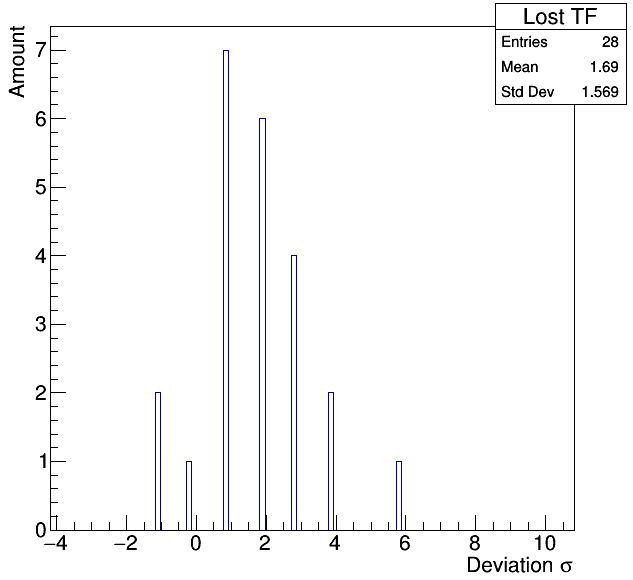
\includegraphics[scale=0.5]{./graphics/ex3_histogram.png}
	\caption{Histogram of the TF loss for ticktime 5}
	\label{fig:Ex3Histogram}
\end{figure}

\newpage

%\section{Ex.1 3 FLPs 18 EPNs}
%\textbf{Ticktime influence on the Blacklist algorithm with one fail-over.}
%\\~\\

%\section{Ex.2 3 FLPs 18 EPNs}
%\textbf{Ticktime influence on the Blacklist algorithm with all but one fail-over.}
%\\~\\

%\section{Ex.3 3 FLPs 18 EPNs}
%\textbf{Ticktime influence on the Blacklist algorithm with all but one-fail over with random sample size.}
%\\~\\

%\section{Ex.1 4 FLPs 24 EPNs}
%\textbf{Ticktime influence on the Blacklist algorithm with one fail-over.}
%\\~\\

%\section{Ex.2 4 FLPs 24 EPNs}
%\textbf{Ticktime influence on the Blacklist algorithm with all but one fail-over.}
%\\~\\

%\section{Ex.3 4 FLPs 24 EPNs}
%\textbf{Ticktime influence on the Blacklist algorithm with all but one fail-over with random sample size.}
%\\~\\

%\section{Ex.4 4 FLPs 24 EPNs}
%\textbf{Ticktime influence on the Blacklist algorithm with all but one fial-over at once.}

\section{Analysis}
\subsection{Comparison to the previous experiment}
Looking at the data from the experiment, the difference is almost negligible. Tables ~\ref{table:DifEx1} , ~\ref{table:DifEx2} and ~\ref{table:DifEx3} show the percentage difference of all the results.

\begin{table}[h!]
\begin{tabular}{| l | l | l | l | l |}
\hline
Ticktime & Raspberry & Xeon & \% Difference & Total \\ \hline
5 & 2.16 & 1.24 & 74.19 & \\ \hline
10 & 2.13 & 1.84 & 15.76 & \\ \hline
15 & 3.08 & 2.16 & 42.59 & \\ \hline
20 & 3.0 & 2.12 & 41.51 & \\ \hline
25 & 3.52 & 2.708 & 29.99 & \\ \hline
30 & 4.32 & 3 & 44.00 & \\ \hline
35 & 4.13 & 3.52 & 17.33 & \\ \hline
40 & 4.56 & 3.76 & 21.28 & \\ \hline
& & & & \textbf{32.19\%} \\ \hline
\end{tabular}
\caption{\% Difference in mean of TFs lost of experiment one.}
\label{table:DifEx1}
\end{table} 

\begin{table}[h!]
\resizebox{\textwidth}{!}{\begin{tabular}{| p{0.1\linewidth} | >{\centering}m{0.8cm} | >{\centering}m{0.7cm} | >{\centering}m{0.7cm} | >{\centering}m{0.7cm} | >{\centering}m{0.7cm} | >{\centering}m{0.7cm} | >{\centering}m{0.7cm} | >{\centering}m{0.7cm} | >{\centering}m{0.7cm} | >{\centering}m{0.7cm} | >{\centering}m{0.7cm} | >{\centering}m{0.8cm} |}
\hline
Lost EPNs & 1 EPN & 2 EPNs & 3 EPNs & 4 EPNs & 5 EPNs & 6 EPNs & 7 EPNs & 8 EPNs & 9 EPNs & 10 EPNs & 11 EPNs & \textbf{Total} \tabularnewline \hline
Ticktime &&&&&&&&&&&& \tabularnewline \hline
5 & 100 & 0 & 0 & 0 & 0 & 50 & 50 & 0 & 33.33 & 33.33 & 25 & 23.08 \tabularnewline \hline
10 & 100 & 50 & 0 & 0 & 0 & 33.33 & 33,33 & 33.33 & 0 & 25 & 40 & 23.53 \tabularnewline \hline
15 & 200 & 0 & 0 & 0 & 33.33 & 33.33 & 0 & 25 & 50 & 40 & 28.57 & 27.50 \tabularnewline \hline
20 & -66.7 & 33.33 & 33.33 & 33.33 & 0 & 25 & 25 & 20 & 40 & 50 & 37.5 & 16.98 \tabularnewline \hline
25 & -63.6 & 33.33 & 0 & 0 & 25 & 25 & 20 & 40 & 50 & 42.86 & 44.44 & 14.52 \tabularnewline \hline
&&&&&&&&&&&& \textbf{20\%} \tabularnewline
\hline
\end{tabular}}
\caption{\% Difference per lost TFs per EPN of experiment two}
\label{table:DifEx2}
\end{table}

\begin{table}[h!]
\resizebox{\textwidth}{!}{\begin{tabular}{| p{0.1\linewidth} | >{\centering}m{0.8cm} | >{\centering}m{0.8cm} | >{\centering}m{0.7cm} | >{\centering}m{0.7cm} | >{\centering}m{0.7cm} | >{\centering}m{0.7cm} | >{\centering}m{0.7cm} | >{\centering}m{0.7cm} | >{\centering}m{0.7cm} | >{\centering}m{0.7cm} | >{\centering}m{0.7cm} | >{\centering}m{0.8cm} |}
\hline
Lost EPNs & 1 EPN & 2 EPNs & 3 EPNs & 4 EPNs & 5 EPNs & 6 EPNs & 7 EPNs & 8 EPNs & 9 EPNs & 10 EPNs & 11 EPNs & \textbf{Total} \tabularnewline \hline
Ticktime &&&&&&&&&&&& \tabularnewline \hline
5 & 0 & 0 & 0 & 0 & 50 & 0 & 0 & 0 & 33.33 & 0 & 20 & 10.34 \tabularnewline \hline
10 & 50 & -33.3 & 0 & 0 & 0 & 0 & 0 & -25 & 0 & 0 & 16.67 & 0 \tabularnewline \hline
15 & -72.7 & 0 & 0 & 0 & 33.33 & 33.33 & 0 & 20 & 20 & 16.67 & 28.57 & -1.92 \tabularnewline \hline
20 & -70 & 0 & 33.33 & 33.33 & 0 & 0 & 25 & 20 & 0 & 14.29 & 33.33 & 1.72 \tabularnewline \hline
25 & -69.2 & 33.33 & 0 & 0 & 0 & 25 & 20 & 40 & 14.29 & 25 & 30 & 2.99 \tabularnewline \hline
&&&&&&&&&&&& \textbf{2.05\%} \tabularnewline
\hline
\end{tabular}}
\caption{\% Difference per lost TFs per EPN of experiment three}
\label{table:DifEx3}
\end{table}

%\subsection{Increasing the numbers of FLPs and EPNs}
